\glsreset{co2hb}
\chapter{Conclusion and Perspectives}\label{chap:conclusion}

\begin{tldrbox}
	
	This last chapter is divided into four parts. The first part briefly summarises the main contributions of this thesis. The second part then outlines the key points that need to be addressed for the future of dye-based thin film transcutaneous \gls{co2} sensing. The third part explores other potential research avenues not directly related to the subject of this doctoral work. Finally, the fourth part concludes this manuscript with a concise bullet-point list of the core ideas of this thesis, along with channels to follow my likely future endeavours.
	
	\tcblower
	
	\hyperref[chap:thin_film]{Previous chapter} \hfill \hyperref[chapter:toc]{Main Table Of Content (TOC)} \hfill \hyperref[chap:biblio]{Next chapter}

\end{tldrbox}

All good things must come to an end, and this doctoral journey is no exception. This final chapter has the delicate task of bringing this thesis to a close, with a dual purpose: briefly summarizing the key contributions made throughout, and highlighting promising research directions for future work. Indeed, as the reader who loves figures would have noticed, the
\begin{center} \includegraphics{0_front_matter/front_figures/tikz/out/frin.pdf}
\end{center}
\noindent{}symbol appears \the\numexpr\value{mfrincounter}-2\relax{} times throughout this manuscript---excluding its introductory and current occurrences, of course---which translates into at least as many open research avenues. Yet, while some of those avenues must be explored to achieve real-word non-invasive transcutaneous \gls{co2} sensing using dye-based thin films, others consist in more fundamental research questions that are only loosely related to the subject of this thesis, or whose answers are not critical to the development of the said sensing scheme. As a result, the perspectives-related part of the present chapter is divided in two, so as to accommodate for this state of affairs.

\section{Main Contributions}

This thesis resulted in four journal articles and one shorter conference communication\cite{dervieux2020, dervieux2022, dervieux2023rate, dervieux2024phase, dervieux2024newcas}, to which the hasty reader is redirected for a rapid overview of the work done. A short glance at the \hyperref[chapter:toc]{table of contents} of this manuscript also gives a good idea of the key aspects of this doctoral thesis. For a brief synopsis, please carry on reading.

\subsection{Context and Early Spectrophotometric Work}

This doctoral work is grounded in a robust clinical and physiological context---Chapter~\ref{chap:intro} and Section~\ref{sect:co2hb:blood_gases}---which offers clear motivations---and even a pressing need---to develop a new generation of transcutaneous \gls{co2} monitors. To do so, two main research avenues were initially envisioned: either \textit{(i)} using a hypothetical change in the absorption spectrum of haemoglobin upon \gls{co2} capture, or \textit{(ii)} measuring the transcutaneous partial pressure of \gls{co2}---\gls{ptco2}---directly, thanks to the diffusion of \gls{co2} through the skin. Haemoglobin spectrophotometry was first investigated---Chapter~\ref{chap:co2hb}---with the initial intention of giving birth to \emph{pulse carbametry}, \ie{} the equivalent of pulse oximetry, but for \gls{co2} instead of \gls{o2}. However, \textbf{the optical properties of \gls{co2hb}---both in absorbance and fluorescence---appeared to be identical to that of \gls{hb} for all practical purposes}. This nevertheless led to a first publication in the Journal of Biomedical Optics to report the absorbance spectra of \gls{o2hb}, \gls{hb}, and \gls{co2hb} in the 235--1000~nm range\cite{dervieux2020}. This spectrophotometric research avenue was then abandoned, and the remainder of the time allocated to this thesis was devoted to the transcutaneous \gls{co2} diffusion pathway.

\subsection{Transcutaneous \texorpdfstring{\gls{co2}}{CO2} Sensing}

With this ultimate goal in mind, a lot of work remained to be done in order to yield a next-generation, clinically usable, \gls{ptco2} sensor:
\begin{enumerate}
	\item The transcutaneous diffusion of \gls{co2} needed to be accurately characterised, in particular with respect to skin temperature. It was also necessary to get a clear picture of the other environmental conditions present at the skin.
	\item These two pieces of information could then be used as guiding factors in choosing an appropriate \gls{co2} sensing technique for transcutaneous measurements.
	\item Having chosen that technique---\ie{} dye-based thin film sensing---several theoretical considerations needed to be put out of the way, and optimising the chemistry of the thin films remained to be done.
	\item Finally, the correlation between \gls{ptco2} and \gls{paco2} also needed to be accurately characterised with respect to skin temperature.
\end{enumerate}
This doctoral work satisfyingly addressed the first two aspects of the above to-do list, partially investigated the third one, and did not have the time to even scratch the surface of the last one---except for indices related to micro-circulation measurements.

\subsubsection{Sensing at the Skin}

Starting with skin properties, a simple model based on Fick's first law was proposed to describe transcutaneous \gls{co2} diffusion---Section~\ref{sect:tcco2:modelling_tc_sensing}. This model led to the definition of a metric called skin \emph{conductivity} towards \gls{co2}, whose primary interest is that it does not depend on the ambient \gls{co2} level nor on the test subject's \gls{ptco2}, as opposed to the transcutaneous \gls{co2} \emph{diffusion rate} used up till now in the literature. A custom skin conductivity sensor allowing for cutaneous temperature regulation was then designed, and later used in a clinical study involving forty participants---Section~\ref{sect:tcco2:frontiers_article}.

Briefly, this study showed that skin conductivity at most doubles from 35 to 44{\degree}C at the wrist and upper arm. This first result is encouraging for the development of next-generation \gls{ptco2} sensors, since it means that \textbf{heating the skin is not mandatory from a response time point of view}, thus potentially enabling wearable sensors. This clinical study also included micro-circulation measurements at the upper arm, showing a doubling of perfusion from non-heated to 35{\degree}C, and a quadrupling from non-heated to 38{\degree}C. This second result is also encouraging, as it gives clues indicating that \textbf{heating the skin is probably not mandatory to guarantee a good \gls{ptco2} / \gls{paco2} correlation either}. This clinical study and the above results led to a publication in the Frontiers in Physiology journal\cite{dervieux2023rate}. Further research was also conducted on cutaneous environmental conditions---Section~\ref{sect:tcco2:skin_conditions}---and revealed that occluded human skin is a humidity-saturated medium, slightly hypoxic, whose temperature can reach over 35{\degree}C under light clothing, and which can exudate a variety of acidic compounds.

\subsubsection{Choosing a \texorpdfstring{\gls{co2}}{CO2} Sensing Scheme}

A massive bibliographic effort was then undertaken to map out the landscape of \gls{co2} sensing, and resulted in the publication of a review journal article in Sensors\cite{dervieux2022}. \textbf{This work, combined with the afore-described cutaneous specificities, led to the selection of dry, dye-based, thin film sensors} among the many state-of-the-art solutions suitable for \gls{co2} sensing---Section~\ref{sect:choos:techno_choice}. The basic chemistry of these thin films was then presented, and optical sensing schemes were also reviewed---Section~\ref{sect:choos:dye_based}---leading to the selection of an \gls{fdlr} sensing scheme.

\subsubsection{Fine-Tuning the Sensing Scheme and Thin-Film Formulation}

While the theoretical foundations for (even dual-frequency) \gls{fdlr} were laid in the late 1990s by a pioneering team at the University of Regensburg\cite{neurauter2000_phd, klimant2001_pap}, the relationship between noise levels---\eg{} additive or phase noises---and error in the estimation of the analyte concentration remained to be demonstrated. What initially appeared to be a simple question about accurate phase estimation from a noisy sinusoidal signal actually took several months to answer, filling over ten pages of equations---Section~\ref{sect:choos:phase_mes}. These relentless efforts were not in vain, however, since \textbf{a formula was finally derived, linking noise levels, sample count, and phase estimation accuracy}---and thus \gls{co2} concentration accuracy in the case of \gls{fdlr} \gls{co2} sensing. The resulting analysis---valuable not only within the specific context of \gls{fdlr} sensing, but in the more general framework of spectral estimation whenever synchronous sampling is possible---has been published in the APSIPA Transactions on Signal and Information Processing\cite{dervieux2024phase}.

Time was then devoted to selecting suitable chemicals for the thin film formulation, both in terms of choosing appropriate polymers and luminophores---Sections~\ref{sect:thin_film:encaps}--\ref{sect:thin_film:select_poly}. In particular, the detrimental influence of \gls{o2} on photobleaching and luminescence quenching was given significant attention, as was the expected impact of water uptake on \gls{hpts} fluorescence intensity, especially regarding its encapsulation into a breathable polymer. A sensing optoelectronics assembly was then designed to probe the thin films that were manufactured using the selected chemicals, demonstrating the \invitro{} feasibility of the technique for \gls{co2} sensing at physiological levels. \textbf{This enabled the validation of the theoretical developments mentioned above regarding phase estimation accuracy}, and led to a short communication at the 2024 NEWCAS conference\cite{dervieux2024newcas}. Additionally, the photobleaching, quenching, and humidity influence phenomena were briefly investigated. While photobleaching should not pose a significant issue in practice, the use of anti-fading agents seems to be an interesting avenue to explore so as to strengthen the resulting thin films. It remains unclear whether the influence of humidity would be an actual problem in real-life transcutaneous applications; however, it is indeed challenging in the lab, where achieving saturating humidity levels has proven relatively difficult.

\section{Short-Term Research Avenues for \texorpdfstring{\gls{co2}}{CO2} Sensing}

This section and the next focus on potential directions for future research, which were split into two categories. In the current section, the emphasis is placed on short-term research avenues that may have a direct---and potentially strong---impact on the development of next-generation \gls{ptco2} sensors. In the next section, by contrast, the focus shifts to other research avenues which may not be critical to explore from a \gls{ptco2} sensing point-of-view, but whose investigation is of a certain scientific interest. Of note, the issues raised in the following subsections were arranged in the same order as they appeared in the main manuscript, \textbf{not} in their order of criticality. Regarding the latter, the aspects of utmost importance for the translation of this doctoral work into an industry-ready \gls{ptco2} sensor are the following:
\begin{enumerate}
	\item finding out if a 35--37{\degree}C skin temperature would be high enough to guarantee a clinically-usable correlation between \gls{paco2} and \gls{ptco2}---Section~\ref{sect:conclusion:paptccorrel},
	\item improving the chemistry of the thin films in order to reduce photobleaching---Section~\ref{sect:conclusion:photobleaching}---and humidity cross-sensitivity---Section~\ref{sect:conclusion:humidity}, and
	\item miniaturising the optoelectronics---Section~\ref{sect:conclusion:miniaturisation}---and moving from a glass to a polymer substrate---Section~\ref{sect:conclusion:substrate}---to perform early \invivo{} tests.
\end{enumerate}

\subsection{\texorpdfstring{\gls{nir}}{NIR} Haemoglobin Spectrophotometry}

As mentioned in the conclusion of the second chapter---Section~\ref{sect:co2hb:conclusion}---some additional haemoglobin absorption spectra were measured in the \gls{nir}. Briefly, the protocol used was the same as that detailed in Section~\ref{sect:co2hb:pulse_carbametry}, with the exception that blood was not diluted, but rather \emph{concentrated}. Indeed, due to the exceedingly low absorbance of haemoglobin species in the \gls{nir}---see Section~\ref{sect:co2hb:hb_spectra}---and in order to achieve reliable spectrophotometric measurements, it has proved necessary  to reach haemoglobin concentrations at least as high as that of human blood. To do so, venous blood was centrifuged and rinsed thrice upon collection to finally keep only the erythrocytes, which were then lysed with ultrasounds, and equilibrated with different gases---\gls{co2}, \gls{n2}, \gls{co}, and ambient air. The absorption spectra of the so-obtained \gls{o2hb}, \gls{hb}, \gls{co2hb}, and \gls{cohb} solutions were then recorded across the full 600-2350~nm range, and the total haemoglobin concentrations of the samples were also measured using a \gls{cnhb} standard.

Unfortunately, due to the significant water absorption in the \gls{nir} and the dilution effects that ensue---also due to a lack of time---the resulting haemoglobin spectra could not be presented in this thesis. It is envisioned to remedy this situation and publish a short paper on the \gls{nir} absorbance of haemoglobin by early 2025. \textbf{Although---and this should be stressed out---a thorough analysis is yet to be done to confirm or refute this early observation, there seems to be no perceivable difference between the absorbance spectra of \gls{hb} and \gls{o2hb} in the \gls{nir}.} Again, this would be expected for the conformational reasons already-mentioned in Section~\ref{sect:co2hb:conclusion}, and would bring yet another nail to the coffin of pulse carbametry. Still, to the best of my knowledge, this would at the same time be one of the few reports of human haemoglobin in the \gls{nir}---see Table~\ref{tab:co2hb:hb_biblio}---and the first one providing tabulated coefficients.

\subsection{\texorpdfstring{\gls{paco2} / \gls{ptco2}}{paCO2 / tcpCO2} Correlation at Low Skin Temperature}\label{sect:conclusion:paptccorrel}

Although \textit{(i)} there is empirical proof that subcutaneous micro-circulation at the upper arm doubles at 35{\degree}C and quadruples at 38{\degree}C compared to baseline---see Section~\ref{sect:tcco2:results}---and \textit{(ii)} there is a sound theoretical framework to explain why this should translate into a good correlation between \gls{paco2} and \gls{ptco2} at those temperatures---see Section~\ref{subsect:tcco2:frontiers:acc_impact}---this correlation remains to be demonstrated experimentally. More specifically, there is---to the best of my knowledge---no report of such correlation below 37{\degree}C, and only Wimberley \etal{} did experiment at this temperature back in 1985\cite{wimberley1985a}. In their study, the authors demonstrated a good agreement between \gls{paco2}\footnote{Actually, they used arterialised capillary blood punctured from the earlobe, which exhibits excellent agreement with arterial blood in terms of \gls{pco2}\cite{zavorsky2007}.} and \gls{ptco2} on a sample of only ten human subjects, making it a relatively fragile piece of evidence. \textbf{This \gls{paco2} / \gls{ptco2} correlation issue at low temperature is, in my humble opinion, one of the strongest remaining locks to the development of wearable \gls{ptco2} sensors.} Indeed, wearable battery-powered sensors cannot afford actively heating the skin for obvious power-consumption reasons, and only the existence of the latter correlation at low temperatures---\ie{} temperatures achievable without active heating---would make their materialisation conceivable, as discussed in Section~\ref{sect:tcco2:frontiers_article}.

\subsection{\texorpdfstring{\gls{co2}}{CO2} Sensing Review Update}

This section is more of a short note---as well as a disclaimer---regarding the technological review presented in Section~\ref{sect:choos:sensors_review}. Indeed, this review is largely adapted from our 2022 Sensors article\cite{dervieux2022}, which was itself based on literature researches from early 2020. It might thus benefit from an update including recently published works on the topic, some of which use novel sensing mechanisms that were not identified in the original review.

Firstly, several publications improved some of the afore-mentioned \gls{co2} sensing mechanisms---\ie{} hydration, reduction, \etc.---which may lead to interesting alternatives to the dye-based thin film approach that is at the heart of this doctoral work. In particular, a team from the University of Eylul published a series of papers on the improvement of \gls{hpts}-based sensors\cite{ongun2021, ongun2023a, oguzlar2023b, yilmaz2024}. Other works include improvements of conductometric\cite{kotbi2022, rath2024}, dye-based\cite{shahid2022, zhang2023atu} or carbamate formation-based\cite{lee2022tur, choi2024} sensors. Another interesting \gls{co2}-sensing route has been proposed using optical probes that exhibit a change in their molecular structure upon reaction with \gls{co2} that differs from a simple carbamation\cite{green2022, zhu2024}. Lastly, it seems that a great deal of research effort is being devoted to \gls{mof} for gas or pH measurement purposes\cite{zhang2023lum, mohammedameen2024}.

Secondly, there has also been a renewed interest for the development of novel \gls{ptco2} sensing modalities in the past few years, following almost forty years of dormancy. With this respect, two strategies emerged: \textit{(i)} that of Grangeat \etal{}\cite{grangeat2023} or Persson \etal{}\cite{persson2023}, using a rate-based approach\footnote{This approach in its simplest form seems doomed to failure, however, as mentioned briefly in the introduction of the above-mentioned NEWCAS article\cite{dervieux2024newcas}, due to the wide variability in skin permeabilities towards \gls{co2} from one subject to another (see Section~\ref{sect:tcco2:results}). One possible solution to overcome this issue could be to implement a per-patient calibration or to use a dual-membrane scheme---as suggested in the early work of Hansen \etal{}\cite{hansen1980}, or more recently by Persson \etal{}\cite{persson2023}.}, and \textit{(ii)} the one proposed in this doctoral work, based on an equilibrium between the subcutaneous tissues and a thin film sensitive to \gls{co2}. This thin film can be dye-based---as proposed by the teams of Cascales \etal{}\cite{cascales2022, cascales2023}, Tufan \etal{}\cite{tufan2022, tufan2023a, tufan2023c}, and Cui \etal{}\cite{cui2024}---redox\cite{ahuja2023}, or potentiometric\cite{jia2024}, for instance. Of note, although other authors proposed equilibrium-based \gls{ndir} sensors---\ie{} similar to that used in Section~\ref{sect:tcco2:frontiers_article}, but waiting for an equilibrium between the tissues and the sensor's chamber---the sensing volumes involved are likely to induce clinically unacceptable lags\cite{li2023non, angelucci2024, elsafoury2024}. Finally, it is also worth mentioning two recent reviews by Tufan \etal{}\cite{tufan2023b} and Bernasconi \etal{}\cite{bernasconi2024} both compiling recent works on the topic of transcutaneous \gls{co2} sensing.

\subsection{Temporal Alternative to \texorpdfstring{\gls{dlr}}{DLR}}

Upon discussions with Wilfried Uhring---the director of this doctoral work---he returned to his old flame for time-resolved ultrafast optical sensing, and put forth the idea that a variant of \gls{tdlr} might be used instead of \gls{fdlr}. Accurate sensing could be achieved by using multiple low intensity pulses---to reduce photobleaching---and then measuring the decay times of the two luminophores involved. The main advantage of doing so is that the emission and reception optical filters may thus be omitted. This may be of particular interest from a large-scale industrialisation point-of-view, since the optical filters are by far the costliest pieces of equipment of the whole sensing optoelectronics. However, this sensing scheme might require more expensive acquisition electronics and should thus be carefully studied from a cost perspective.

\subsection{Photobleaching Investigations}\label{sect:conclusion:photobleaching}

Although the photobleaching of \gls{rudpp} and \gls{hpts} is already relatively low---below 2\% for two weeks of service, taking one measurement per minute---further reducing its magnitude may still prove beneficial in order to improve the sensor's accuracy. In particular, the use of anti-fading agents such as \gls{dabco} seems promising, especially for \gls{hpts}---see Section~\ref{subsect:thin_film:experimental:pbl:hpts}. Studying the photobleaching mechanisms and pathways for both luminophores more deeply is also mandatory to devise appropriate measures to mitigate the said phenomenon. \textbf{Most critically, knowing the dynamics of the phenomenon, as well as its dependence on the luminophores' concentrations and illumination power would allow a compromise to be made between these parameters and the illumination duration}---through the sample count $N$---as evoked in Section~\ref{subsect:thin_film:experimental:newcas}. Since polymer-dye interactions can also influence photobleaching---see Section~\ref{subsect:thin_film:experimental:pbl:rudpp}---it could also be interesting to further investigate the use of different polymers for both luminophores.

\subsection{Alternative Luminophores}

Despite the significant research efforts that were put into selecting suitable luminophores for the envisioned \gls{fdlr} application---see Section~\ref{sect:thin_film:select_lumino}---\gls{hpts} and \gls{rudpp} may not be the absolute optimal choice. Indeed, their selection was performed on a subset of the myriad of available off-the-shelf luminophores, and other dyes might have been benchmarked. In particular two main directions could be followed: \textit{(i)} other long-lived organometallic complexes could be envisioned to replace \gls{rudpp} among those proposed by Wang \etal{}\cite[Sect.~6.2]{wang2014wolfbeis}, taking care to keep only the ones that exhibit a relatively low sensitivity towards oxygen, \textit{(ii)} in line with the previous section, photobleaching could also be taken into account for luminophore selection---in addition to the cost / luminance / pH-sensitivity analysis already performed. The main issue with this latter option, however, is that photobleaching data are scarcely available in the literature for the said fluorophores. This state of affairs---combined with the photobleaching dependency towards encapsulating polymer, concentration, \etc.---unfortunately makes objective comparisons between one luminophore and the next exceedingly difficult, if not impossible, potentially requiring thorough experimentations to yield meaningful, exploitable figures.

\subsection{Humidity Cross-Sensitivity}\label{sect:conclusion:humidity}

The manufactured thin films demonstrated a major cross-sensitivity towards humidity---see Section~\ref{sect:thin_film:experimental:humid}. While it is not certain at the time of writing whether this would translate into an actual issue for real-world \gls{ptco2} sensing, it is definitely an issue in the lab, wherein reaching humidity levels close to saturation proved to be exceedingly difficult. The reasons for this cross-sensitivity are also unclear at the time being, with two mutually compatible hypotheses put forth: \textit{(i)} there are not enough water molecules available in the \gls{hpmc} thin film at below-saturation humidity levels, or \textit{(ii)} the humidity level has a strong impact on the optical properties of the \gls{hpmc} thin film. This issue should definitely be addressed swiftly, in order to devise appropriate mitigation strategies. In particular, changing the polymer, adding more plasticisers, phase transfer agent, and investigating the McMurray hypothesis all seem possible avenues for future research.

\subsection{Changing the Substrate}\label{sect:conclusion:substrate}

For \invivo{} use, \textbf{the manufactured sensing thin films need to switch from a rigid glass substrate to a more flexible one, to conform to the curved organic shapes of the human body}. In contrast with most of the other difficulties encountered in this doctoral work, this issue should be relatively straightforward to address. As mentioned in Section~\ref{subsect:choos:review:dye_based}, both \gls{pen} and \gls{pet} make good candidates for replacing glass: they exhibit a good barrier function towards \gls{co2} when used in thicknesses of about 100~\textmu{}m, are optically clear, flexible, inexpensive, and do not exhibit any significant fluorescence upon 450~nm excitation when compared to the added luminophores\cite{ouchi2007}. Additionally, some tests were already performed in the lab, demonstrating good wettability and film-forming ability of both \gls{pen} and \gls{pet} with respect to \gls{rudpp} / \gls{dmf} / \gls{pan} and \gls{hpts} / \gls{hpmc} / water / ethanol mixtures, and good adhesion of the films upon drying.

\subsection{Miniaturising the Optoelectronics}\label{sect:conclusion:miniaturisation}

With the same \invivo{} sensing objective in mind, \textbf{miniaturising the optoelectronics presented in Section~\ref{sect:thin_film:opto_elec} will be mandatory to make it wearable-embeddable}. This aspect is currently being investigated, and is closer to an engineering work than to an open research question, even if achieving an optical design of about 1~cm$^3$ is still challenging. The envisioned optical design uses smaller \gls{led} and photodiode as the above-presented ones, two interferometric excitation and emission filters, and two ball lenses\footnote{Precise references are not given since developments are still ongoing.}. Including a protective glass cover, the overall dimensions of this optical setup is about $13\times7\times6$~mm. In a first \invivo{}-ready prototype, it is envisioned to use it with the legacy electronics presented in Section~\ref{sect:thin_film:opto_elec}, potentially replacing Thorlabs' \gls{tia} by a custom one offering better performance.

\subsection{Develop a Solid Chemical Background}\label{subsect:conclusion:solid_chemistry}

This last point involves substantial work, aiming at developing a consistent theoretical chemical framework for the design of dry dye-based thin films. Indeed, although the chemistry of wet dye-based thin films relies on the classical theory of aqueous solutions and works relatively well in practice\cite{vurek1983, he1995, degrandpre1999}, there is currently no satisfactory equivalent for dry polymer thin films, in particular with respect to phase transfer agent concentration, or dye-polymer interactions. Admittedly, the approach usually adopted in the literature---\ie{} considering that wet chemistry also takes place in dry thin films, as presented in Section~\ref{sect:choos:dye_based:chemistry}---fits remarkably well with experimental data, resulting in a linear relationship between the \gls{co2} concentration and the ratio of fluorescence intensities $I_0/I$ in a ratiometric scheme\cite{borisov2007, chu2008, chu2009}, or in a rational relationship between the \gls{co2} concentration and the measured phase shift in an \gls{fdlr} scheme\cite{burke2006, cajlakovic2009}. Yet, there is to date no theoretical background to satisfactorily explain the influence of phase transfer agent concentration nor embedding polymer choice on the response of dry thin films sensors. To the best of my knowledge, only three papers tried to investigate the influence of the concentration in quaternary ammonium anion\cite{malins1998, fernandezsanchez2007, fernandezramos2018}, and all of them settle for experimental observations without theory to quantitatively back them up.

\begin{figure} % script ch_f_pkr
	\centering
	\includegraphics{1_main_matter/conclusion_figures/tikz/out/chemistry_combined.pdf}
	\caption[Influence of the \pKa{} of the pH-sensitive dye on the sensor's response towards \gls{co2}.]{Influence of the \pKa{} of the pH-sensitive dye A$^-$ / AH on the sensor's response towards \gls{co2}. \textbf{Left:} relationship between \gls{pco2} and the concentration in the anionic form of the pH sensitive dye, \ce{A^-}. The grey area corresponds to the physiological 40--80~mmHg \gls{paco2} range, while $\delta$[A$^-$] and its relative variant $\delta$[A$^-$]$_\text{rel}$ correspond to \ce{[A^-]} variations across it. In this case [Q$^+$] = [A$^-$] + [AH] was set to 1~mM. \textbf{Right:} influence ot the total dye / phase transfer agent concentration and \pKa{} on the relative \ce{A^-} concentration across the 40--80~mmHg range.}
	\label{fig:conclusion:chemistry_combined}
\end{figure}

\begin{figure} % script phimes_f_pkr (ou qqc du genre)
	\centering
	\includegraphics{1_main_matter/conclusion_figures/tikz/out/chemistry_phi.pdf}
	\caption[Influence of the \pKa{} and dyes ratio on the sensor's response towards \gls{co2}.]{Influence of the pH-sensitive / reference dyes ratio and of the \pKa{} of the pH-sensitive dye on the sensor's response towards \gls{co2}. \textbf{Left:} relationship between \gls{pco2} and the measured phase shift as a function of the pH-sensitive / reference dyes ratio. In this case [Q$^+$] = [A$^-$] + [AH] was set to 100~\textmu{}M, the probing frequency (\gls{fdlr} scheme) was set to 80~kHz and typical literature values were taken for the optical properties of \gls{hpts} for the pH-sensitive dye, and \gls{rudpp} for the reference dye. \textbf{Right:} influence ot the total dye / phase transfer agent concentration and \pKa{} on the $\varphi_{mes}$ variation across the 40--80~mmHg range.}
	\label{fig:conclusion:chemistry_phi}
\end{figure}

To try and make up for this lack of understanding, I started from Equation~\ref{eq:choos:dye_based:chemistry:dry_aah_unbuff}, \ie{}
\begin{equation}
	\ce{pCO_2 = \frac{K_A}{K_{13}}}\cdot \frac{\left(\ce{[Q^+] - [Q^+A^-.$(x-1)$H_2O]}\right)\cdot\left(\ce{\mathcal{C}_A - [Q^+A^-.$(x-1)$H_2O]}\right)}{\ce{[Q^+A^-.$(x-1)$H_2O]}}
\end{equation}
and strived to link the concentrations in \ce{Q^+}, pH-sensitive and reference dyes, the \gls{pco2}, and the \pKa{} of the pH-sensitive dye, with the relative variation in the concentration of the anionic form of the pH-sensitive and---more importantly---the resulting phase shift caused by a variation of \gls{pco2}. This analysis led to simulation results akin to those presented in Figures~\ref{fig:conclusion:chemistry_combined} and \ref{fig:conclusion:chemistry_phi}, but it was not included in this thesis for two main reasons: at first, this manuscript is already quite substantial, and this analysis would have made it even longer, not to mention the amount of time necessary to properly typeset it, a time I was running short of. Secondly, I do not have any piece of experimental evidence to back up this work, making it little more than a pipe dream at the time of writing. That being said, the upside of the coin is that \textbf{there is room for a future research program aiming at building an experimentally-supported theoretical framework, which would make designing dry thin film sensors somewhat less like walking in the dark.}

\section{Other Open Avenues}

The other research avenues presented in the following sections are clearly not essential for the improvement of the dye-based thin film \gls{co2} sensors on which this thesis focuses. Still, they constitute interesting research questions, whose answer might bring further insights and a better understanding of the phenomena underlying the above-presented work.

\subsection{Blood Carbamate Formation}

As mentioned in Section~\ref{subsect:co2hb:co2_transport:carbamates}, there seems to be a lack of a satisfactory model to quantitatively relate the blood \gls{pco2} with its \gls{co2hb} concentration---\ie{} with the amount of \gls{co2} present as carbamate haemoglobin compounds. The existence of such a model would allow for the expression of the whole blood carbamate \gls{co2} content as a function of its \gls{pco2}, potentially also including the \gls{23dpg}, bicarbonate ions, and haemoglobin concentrations, as well as blood pH. Although deriving such a model might not be vital from a clinical point-of-view, it might still be interesting to better understand haemoglobin \gls{co2} binding, and more generally blood gases transport, therefore providing valuable insights from a physiological viewpoint.

\subsection{\texorpdfstring{\gls{co2}}{CO2} Diffusion Model}

The diffusion model that was introduced in Section~\ref{sect:tcco2:modelling_tc_sensing}---while allowing for useful derivations and relatively easy skin conductivity measurements---is rather simplistic, modelling the skin as a single membrane, and the tissues as an ideal \gls{pco2} source. As a result, this model does not correspond to any physical reality. In particular, as first mentioned in Section~\ref{sect:tcco2:model} and later emphasised in Section~\ref{sect:tcco2:k_metric_choice}, the thickness of the model's skin membrane does not correspond to the real-world thickness of the \textit{stratum corneum}. It might thus be interesting---in order to yield a more interpretable model closer to the histological reality of skin structure---to separately study the skin conductivities of different skin layers. In particular, such modelling could allow for the prediction of skin conductivity from a given subject's age, since age strongly influences the \textit{stratum corneum}'s thickness\cite{branchet1990}, and this thickness strongly influences skin permeability\cite{scheuplein1976}.

However, to develop such a model, it would be mandatory to have the ability to measure the actual subcutaneous \gls{pco2} at the chosen conductivity measurement site and temperature. Indeed, as noted in Section~\ref{sect:tcco2:k_metric_choice}, the reference \gls{ptco2} monitor that we used could not be set at temperatures lower than 41{\degree}C. This led to conductivity values slightly over-estimated, and is thus not satisfactory from a metrological point-of-view. In particular, in order to develop the afore-mentioned model \invivo{}---\ie{} without having to skin the subjects, but rather by gently peeling their skin with tape, for instance---it would be necessary to have a temperature-regulated \gls{ptco2} monitor capable of low temperature measurement. Of note, in this latter case, the aim of this \gls{ptco2} monitor would be to measure the true subcutaneous \gls{pco2}, and not a proxy for the \gls{paco2}---as is usually done by heating the skin above 41{\degree}C.

\subsection{Sole of the Transcutaneous \texorpdfstring{\gls{co2}}{CO2} Conductivity Sensor}

As noted in Section~\ref{subsect:tcco2:skin_surface}, both \textit{(i)} the shape of the sole of the sensor that was used to measure skin conductivity towards \gls{co2}, and \textit{(ii)} the skin elasticity can affect the exchange surface between the sensor and the skin. This is illustrated sketchily in Figure~\ref{fig:conclusion:sole_shape}, Left. Each circular hole in the sensor's sole will create a small dome of skin, which will have a surface $S$ that deviates from its ideal value of $\pi\cdot R^2$ with increasing skin curvature. This curvature itself depends on the radius of the hole---$R$---on the mechanical properties of the skin, and on the sensor's application force. As can be seen in the a--c parts of the figure, the change in cutaneous exchange surface between an ideal---\ie{} perfectly flat--and worst---\ie{} perfect half-sphere---cases can result in up to a twofold variation. Since $S$ is then used directly to compute the skin conductivity towards \gls{co2} $K$---see Equation~\ref{eq:tcco2:k_effective_calc}---this variation on $S$ directly affects the latter\footnote{In actuality, there is no reason why the shape of the skin dome should be spherical, it could be closer to the surface generated by rotating a catenary around its axis for relatively small---\ie{} a few millimetres---holes. Enlarging the hole leads to a flattening of the dome, as represented in Figure~\ref{fig:conclusion:sole_shape}, Right, because the bond between the skin and the underlying tissues prevents the former from bulging out too much in the centre of the hole.}.

\begin{figure}
	\centering
	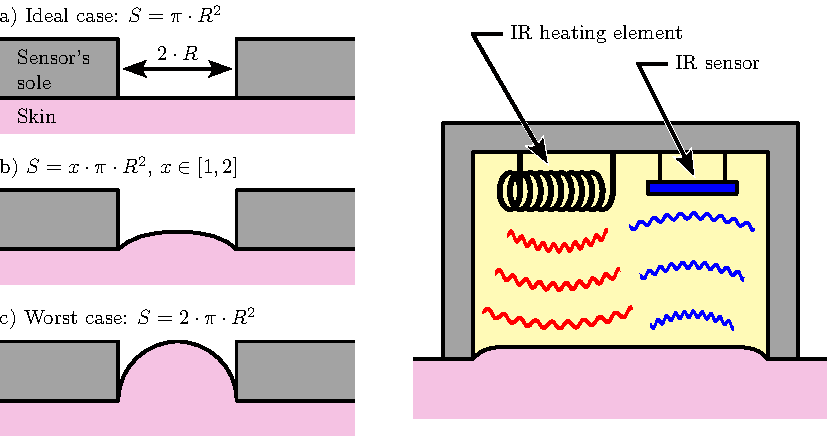
\includegraphics{1_main_matter/conclusion_figures/sole_dome_converted.pdf}
	\caption[Influence of skin elasticity on dome formation, and alternative heating scheme.]{\textbf{Left:} cross-section view of the dome formation effect. Depending on several factors such as the skin elasticity or temperature, the hole radius value $R$, and the sensor's contact force, the dome can be more or less convex. The two extreme situations a and c correspond to a perfectly flat, or a hemispheric shape of the skin surface underneath the hole. \textbf{Right:} an alternative heating method, using a radiative heating system and a single big hole in the sensor's sole, instead of a conductive heating system and multiple holes, as was the case in Section~\ref{sect:tcco2:frontiers_article}.}
	\label{fig:conclusion:sole_shape}
\end{figure}

Yet, as discussed in Section~\ref{subsect:tcco2:skin_surface}, this is no easy problem to remedy: there is a compromise to be made between the shape of the sensor's sole and its thermal efficiency. More specifically, using a single very large hole is likely to mitigate the dome formation effect, as illustrated in Figure~\ref{fig:conclusion:sole_shape}, Right. However, without adapting the heating system---\ie{} if the heat is brought \emph{conductively} by the sensor's sole itself, as presented in Section~\ref{subsect:tcco2:mat_sensor}---the skin at the centre of the hole would likely be cooler than the sole---\ie{} it would be cooled at the \gls{nh} temperature by the subcutaneous blood flow. One possible way to address this would be to implement a \emph{radiative} heating system coupled to an infrared remote sensor for accurate thermoregulation of the skin surface, as presented in Figure~\ref{fig:conclusion:sole_shape}, Right. Such a design could therefore be envisioned for future quantitative studies of skin conductivity towards \eg{} \gls{co2} as a function of the skin temperature.

\subsection{Influence of Occlusion on Skin \texorpdfstring{\gls{co2}}{CO2} Conductivity}

Observed if only through the whitening and swelling of the skin under a plaster, occlusion does have an impact on the properties of human skin. More specifically, occlusion and the hydration that ensues have long been known to strongly influence the skin barrier properties\cite{zhai2002}. In the case of \gls{co2}, the influence of skin occlusion on the transcutaneous diffusion rate has been studied by several authors\cite{frame1972, king1978, faergemann1983}---see Section~\ref{subsect:tcco2:gas_tightness}---and these early works demonstrated much higher \gls{co2} exhalation rates for long-term---\ie{} days---occluded skin, as compared to its basal state. It could therefore be interesting to extend the study performed in Section~\ref{sect:tcco2:frontiers_article} to occluded skin. Of note, since the sensor presented in Section~\ref{subsect:tcco2:mat_sensor} is relatively unpractical to keep for several hours---not to mention days---it could be envisioned to first place an occlusive dressing on the skin of human subjects, and only then---\ie{} after several hours or days---remove it and replace it with the above-mentioned sensor for conductivity measurements.

\subsection{Conductivity Variability Factors}

Another aspect that could deserve further attention is the wide variability---\ie{} about threefold variations, see Section~\ref{subsect:tcco2:results:ks}---observed in measured skin conductivities towards \gls{co2}. Age- and sex-based analyses were conducted using a \gls{manova} but yielded non-significant results (p-values above 0.05, even without Bonferroni correction). The source of variability from one subject to another thus remains unclear: at low temperature, it could be related to the afore-mentioned gap between the actual subcutaneous \gls{pco2} and that measured by the \gls{ptco2} monitor. However, this gap should no longer exist at 41{\degree}C, for instance, whereas the wide variability observed persists at this temperature. Perhaps conducting further studies including more participants could clarify this, or perhaps the observed variability is inherent to this metric.

\hl{Hum, je suis un peu à cours d'inspiration, je trouve ça pas fou la variabilité qu'on observe, mais je sais pas vraiment quoi en faire non plus.}

\subsection{Working Principle of Metal Oxide Sensors}

Discussed in Section~\ref{subsect:choos:review:metal_oxide}, the working principle of metal oxide thin film gas sensors remains relatively obscure. Indeed, several mechanisms seem to take place concurrently in such films: a purely conductive effect due to the depletion of lattice electrons upon \gls{co2} adsorption---which may itself be mono-, bi-, or tridentate\cite{usseinov2019}, and also depends on which adsorption plane is considered\cite{tang2013}---and a semi-conductive effect depending on the dopant used\cite{niu2004, sato2007, ra2010}. These two phenomena, combined with the virtually infinite possibilities of doping elements and their mass fractions, make any prediction regarding the sensing performance of any given sensor formulation quite adventurous, at best. Additionally, most \textit{ab initio} simulations available in the literature considered only a uniform lattice---\ie{} without the addition of doping elements. It would therefore be interesting to see further research aiming at aggregating the existing studies on metal oxide sensing into a single theoretical framework, taking into account the many possible planes, adsorption modalities, doping substances, and grain boundaries effects. Such a framework would in turn be exceedingly useful for the development of more sensitive / selective \gls{pco2} sensors, and any step in this direction---however small---would be relevant in moving away from the trial-and-error approach used to date.

\subsection{\texorpdfstring{\gls{drs} for \gls{ptco2} Sensing}{DRS for tcpCO2 Sensing}}

Briefly mentioned in Section~\ref{subsect:choos:pot:drs}, \gls{drs} seems to be an interesting avenue for investigation, as it could potentially allow direct transcutaneous \gls{co2} measurements---\ie{} without having to resort to an approach based on equilibrium with an external detection medium, as is the case with dye-based thin film sensors. However, two major challenges still hinder the application of \gls{drs} to \gls{ptco2} monitoring. First, \gls{drs}-based \gls{co2} sensing uses wavelengths in the 1--4.3~\textmu{}m range\cite{domjan1994, schaden2004}. Water's very high absorbance at these wavelengths---\ie{} over 5cm$^{-1}$ above 1380nm, and over 10cm$^{-1}$ above 1850nm\cite{kou1993}---would likely attenuate any \gls{drs} signal by orders of magnitude, making their detection significantly more difficult than in a classic pulse oximetry setup\footnote{For the record, whole blood absorbance is below 10~cm$^{-1}$ in the 650--1000~nm range usually used for pulse oximetry measurements\cite{bosschaart2014}.}. Second---and this comes as a direct consequence of the limited penetration depth of not-so-near infrared radiations into human tissues---it is not known at the time being whether a pulse signal could be retrieved when using \gls{drs} on living tissues in the above-mentioned wavelengths range. Would it be the case, however, the whole theoretical background developed for pulse oximetry would likely be usable for \gls{drs}-based \gls{ptco2} sensing. Encouragingly, one clue that \gls{drs} \emph{could} work is the fact that whole blood absorbance in the 1000--2500~nm range is comparable to that in the 500--600~nm range\cite{bosschaart2014}, which yields an exploitable green \gls{ppg} signal\footnote{Even if---as always---things may not be that simple, since the pulsatile waveform of green \gls{ppg} signals is thought to originate from \emph{venous} blood put into motion by more deeper arteries, and not by arterial blood \textit{per se}\cite{kamshilin2017}.}. Yet, one remaining challenge for \gls{drs} \gls{ptco2} sensing is the lack of low-cost available optical sources and detectors in the 1--4.3~\textmu{}m range\footnote{For instance, infrared \glspl{led} references above 1300~nm available at \href{https://web.archive.org/web/20240929023831/https://www.thorlabs.com/newgrouppage9.cfm?objectgroup_id=2814}{Thorlabs}, \href{http://web.archive.org/web/20241008134940/https://fr.rs-online.com/web/c/afficheurs-et-optoelectronique/led-diodes-electroluminescentes/leds-infrarouges/?applied-dimensions=4291007801\%2C4291007802\%2C4291453920&pn=1&sortBy=P_breakPrice1&sortType=ASC&group_by_tn=false}{Radiospare}, and \href{http://web.archive.org/web/20241008130626/https://www.roithner-laser.com/pricelist.pdf}{Roithner} easily cost several (tens of) euros. For comparison, ordinary (infra)red \glspl{led} can cost as low as a few cents---\eg{} LTST-C170EKT (Lite-On, Taiwan), \href{http://web.archive.org/web/20241009074635/https://fr.rs-online.com/web/p/leds/1689711}{$\sim$3~ct\euro/pc}.}, which could hamper its industrialisation. Overall, the \gls{drs} research avenue appears promising, and continued efforts in this direction could unlock new transcutaneous sensing modalities.

\section{Epilogue}

The time has now come to bring this long journey through the lands of transcutaneous \gls{co2} sensing to an end, and I sincerely hope that you enjoyed reading this manuscript as much as I enjoyed conducting the associated research. You are now hopefully well aware of the nuts and bolts underlying practical transcutaneous \gls{co2} sensing, and of the limitations that still hinder its large-scale commercial development. In particular, I trust that my efforts to provide you with detailed insights throughout these dense pages, while trying to maintain an educational tone and including appropriate references for further exploration, have not been in vain: this was mandatory  to ensure you could navigate the multi-disciplinary nature of this doctoral work.

\begin{keypointbox}
	In a nutshell, the key takeaways of this thesis are the following:
	\begin{itemize}
		\item[--] The transcutaneous diffusion of \gls{co2} through human skin and the measurement of the resulting \gls{ptco2} appears to be a promising approach for having a proxy for \gls{paco2}.
		\item[--] However, current monitors are expensive, bulky, non battery-powered, and drifting. Dye-based thin film sensors could alleviate most of these issues, but battery-powered sensors still require two conditions to be fulfilled:
		\begin{enumerate}
			\item[--] skin permeability must be sufficiently high at low temperature to ensure a reasonably fast sensor response, this was proven to be the case.
			\item[--] there should be a good correlation between \gls{paco2} and \gls{ptco2} at low temperature, this is yet to be demonstrated.
		\end{enumerate}
		\item[--] Using an \gls{fdlr} sensing scheme with dye-based sensors enables reaching an arbitrarily good accuracy on \gls{pco2} measurements.
		\item[--] The dye-based sensors manufactured in this thesis still suffer from several shortcomings---humidity cross-sensitivity and photobleaching, in particular---that require further investigation.
	\end{itemize}
\end{keypointbox}

As a final note, I have no intention of stopping there, if only to publish the above-mentioned infrared absorption spectra of various haemoglobin species. After six years of having dedicated myself to this doctoral work, I am indeed more than ever motivated to bring dye-based thin film transcutaneous \gls{co2} sensing from the lab to the field. If you are interested in following my future works, feel free to follow me on \href{http://web.archive.org/web/20241009063754/https://www.researchgate.net/profile/Emmanuel-Dervieux-2}{ResearchGate} or \href{https://web.archive.org/web/20241009063905/https://scholar.google.fr/citations?user=DCR_h9YAAAAJ&hl=fr}{Google Scholar}. You may also \href{mailto:emmanuel.dervieux@gmail.com}{contact me} directly for further discussions.